\documentclass[]{llncs}   % list options between brackets

\usepackage{color}
\usepackage{graphicx}
\usepackage{subcaption}
\usepackage{amssymb}
\usepackage{standalone}
\usepackage{pgfplots}
\usepackage{amsmath}
\usepackage{tikz}

\usepackage{listings}

\usepackage{hyperref}

\usepackage{systeme}

\usepackage{enumitem}

\usepackage{float}

\def\shownotes{1}
\def\notesinmargins{0}

\ifnum\shownotes=1
\ifnum\notesinmargins=1
\newcommand{\authnote}[2]{\marginpar{\parbox{\marginparwidth}{\tiny %
  \textsf{#1 {\textcolor{blue}{notes: #2}}}}}%
  \textcolor{blue}{\textbf{\dag}}}
\else
\newcommand{\authnote}[2]{
  \textsf{#1\textcolor{blue}{ #2}}}
\fi
\else
\newcommand{\authnote}[2]{}
\fi

\newcommand{\knote}[1]{{\authnote{\textcolor{green}{Alex notes:}}{#1}}}
% type user-defined commands here

\usepackage[T1]{fontenc}
\usepackage{xcolor}

\definecolor{dkgreen}{rgb}{0,0.6,0}
\definecolor{gray}{rgb}{0.5,0.5,0.5}
\definecolor{mauve}{rgb}{0.58,0,0.82}

\pgfplotsset{compat=newest, table/search path=figures}

\begin{document}

\title{On Contractual Money}

\author{Alexander Chepurnoy, Amitabh Saxena}
\institute{Ergo Platform \\\email{\{kushti,amitabh123\}@protonmail.ch}}

\maketitle

\begin{abstract}
	
It is common to consider functions of money as a medium of exchange, store of value and unit of account. 
In this work we highlight yet another function of money, namely as a unit of contract execution. Historically, there has always been an implicit paper contract behind money. However, with the rise of cryptocurrencies, we now have `programmable money', where it is easy to bind digital assets to an explicit contract. We use the term {\em contractual money} to refer to digital money with a usage contract in the form of executable code. In the first and still the most popular cryptocurrency, Bitcoin, a coin is bound to a contract that combines
statements about secrets and predicates on the blockchain. We note that with certain context extensions, including the spending transaction itself, it becomes possible to implement contractual money. We demonstrate this via two examples using Ergo, a cryptocurrency like Bitcoin. 
In the first example, a private scrip is issued for a microcredit use-case and a contract enforces the borrower to spend the money only as described in the contract (for instance, at least 50\% of the money should be used for buying equipment). 
In the second example, money is issued by a local government to promote local economy. To achieve this, the government pays for communal works at the rate of one token per hour, with each token backed by a fixed amount of national currency. The tokens can be spent in arbitrary ways, but can only be exchanged for national currency by a local producer. 
We also review the famous Woergl experiment of 1934, where according to data published, the main reason for success was not the demurrage component of the Woergl money. Rather, the experiment was a scheme to convert local tax debts into communal works, with demurrage speeding up~(and, to some degree, enforcing) the process.
We conclude by describing a {\em Local Exchange Trading System} (LETS) implemented on top of the Ergo blockchain. To the best of our knowledge, this is the first implementation of LETS using a blockchain.
 
% This is simple enough to work with paper based contracts but digital implementations allow enhanced contracts with additional possibilities. We also review the famous Woergl experiment, where, according to data published by Von Muralt in 1934, the main reason for success was not the demurrage component of the Woergl money. Rather, the experiment was a scheme to convert local tax debts into communal works, with demurrage speeding up~(and, to some degree, enforcing) the process. We conclude by describing a {\em Local Exchange Trading System} (LETS) contract implemented on top of the Ergo blockchain. To the best of our knowledge, this is the first implementation of LETS using a blockchain.

%The second example is a Local Exchange Trading System (LETS), where money in the form of tokens is issued by a local government to promote the local economy. The tokens can be spent in arbitrary ways, but can only be exchanged for national currency by a local producer. To the best of our knowledge, this is the first implementation of LETS using a blockchain.
	
\end{abstract}

\section{Introduction}
\label{sec-intro}
 
Bitcoin~\cite{Nakamoto2008} was introduced in 2008 by Satoshi Nakamoto as a peer-to-peer currency. Its ledger, referred to as a blockchain, is a fully replicated database across the entire network of peers and is updated without a trusted
party or expensive coordination as long as a majority of the peers solving a proof-of-work puzzle are honest.

Originally, digital coins~(of arbitrary denomination) in the Bitcoin ledger were associated with public keys. That is, in order to spend a coin, the owner of the private key corresponding to the public key of the coin should provide a signature for a spending transaction, and validity of the signature could be checked by Bitcoin peers using the public key~(and the spending transaction).
Soon after launch, Bitcoin adopted some programmability allowing a coin is bound to a contract instead of just a public key. A contract combines statements about secrets~(such as ``provide proof of knowledge of private key'') with predicates on blockchain state. In order for validation in a peer-to-peer network without trusted authority, a transaction cannot reference data external to the blockchain because the only data that peers can agree upon when verifying a transaction is the block containing this transaction and blockchain before this block.

A popular trend of cryptocurrencies, which started with Bitcoin in 2009, brought two new exciting features.
Firstly, a cryptocurrency is decentralized, which means that, at the very least, its minting process is permissionless.
Secondly, cryptocurrencies allow programmability to some extent; unlike ordinary coins or notes in the physical world, or the digital representation of fiat money in bank accounts, the coins in Bitcoin are protected by a guarding script. 

Using this concept, we can define a new function of money in addition to the usual ones such as a medium of exchange, store of value, unit of account, and so on. That is, money can act as units of contract execution.

This function implicitly existed since the very early days in money's history. A very clear historical example of paper money associated with a contract is Hundis~\cite{martin2009hundi}. A modern example could be found in
maternity capital in Russia: the government gives a certificate associated with some amount of national fiat currency~(rubles) to mothers of two and more children. Unlike fiat currency, the maternity capital money can be spent only for particular expenses, such as children's education or housing improvement.

However, with cryptocurrencies it becomes easy to make a digital coin whose use cases are
explicitly bounded by a contract in form of executable code stored in the coin itself.

Bitcoin first made that move with a simple scripting language named Bitcoin Script which allows some programmability: a coin could be spent if its protecting script, given arguments provided by spending transaction (along with the height and timestamp of the block provided by the miner) evaluates to $true$. A newer cryptocurrency, called Ergo~\cite{ergowp}, goes a step further, with the spending transaction~(along with other additional
fields) fully projected into the execution context. This enhancement allows even Turing-complete
contracts~\cite{chepurnoy2018self}. In financial applications, it allows creation of a coin which could be spent only by
a transaction that creates another coin with specific properties. In the same fashion, a coin may require a chain of
transactions, or a coin may create a family of coins with specific properties. Thus, it is possible to create contractually bound money (i.e., tokens on the Ergo blockchain) with many possible states. 

The main distinguishing point of contractual money is the embedding of the contract, which existed externally (in form of laws, corporate terms, informal and often implicit person-to-person agreements), directly into the unit of money. Thus, money created with a specific contract enforces its users to follow its rules precisely. Other functions of money (medium-of-exchange, store-of-value, unit-of-account) could be encoded in the contract and thus become secondary.

The paper is organized as follows. Section~\ref{sec-txmodel} describes transactional model of Bitcoin and Ergo. We then  provide a few motivating use-cases for contractual money. Section~\ref{sec-microcredit} provides an example of a one-time microcredit system. Section~\ref{sec-combination} sketches a currency which combines properties of time and local currencies. Section~\ref{sec-worgl} reflects on the famous W\"{o}rgl experiment from a contractual money point of view. Section~\ref{sec-lets} describes two possible Local Exchange Trading System (LETS) implementations on top of the Ergo blockchain, one with a trusted committee and the other with cryptocurrency collaterals to secure debts. We give some concluding points in Section~\ref{sec-conslusion}.


\section{Key Contractual Aspects of Bitcoin and Ergo}
\label{sec-txmodel}

In Bitcoin, a `coin' contains some quantity of tokens known as {\em satoshis}. All coins are stored in short-lived immutable objects called {\em Unspent Transaction Outputs} (UTXOs). 
A UTXO contains an {\em amount} representing the quantity of tokens locked in it and an {\em locking script} representing the requirements under which the tokens may be spent (for instance, it can require a signature on the transaction). Thus, a UTXO can be thought of as a locked box with some tokens inside and the act of spending the UTXO can be thought of as unlocking the box.
The actual state of Bitcoin then is the entire UTXO set. 

A transaction modifies this state by spending existing UTXOs as {\em inputs} and creating new ones as {\em outputs}. 
Bitcoin transactions adhere to a weak conservation law: the total number of tokens in the outputs may be less than or equal to that in the inputs (the exception is a reward transaction that generates new tokens).

Each input UTXO must be accompanied by an {\em unlocking script} that convinces everyone that the condition specified by the locking script is satisfied. For instance, this can be a signature on the transaction. Both scripts executed together determine determine the transaction's validity.
Figure~\ref{fig1} shows how a Bitcoin transaction works.
\begin{figure}
	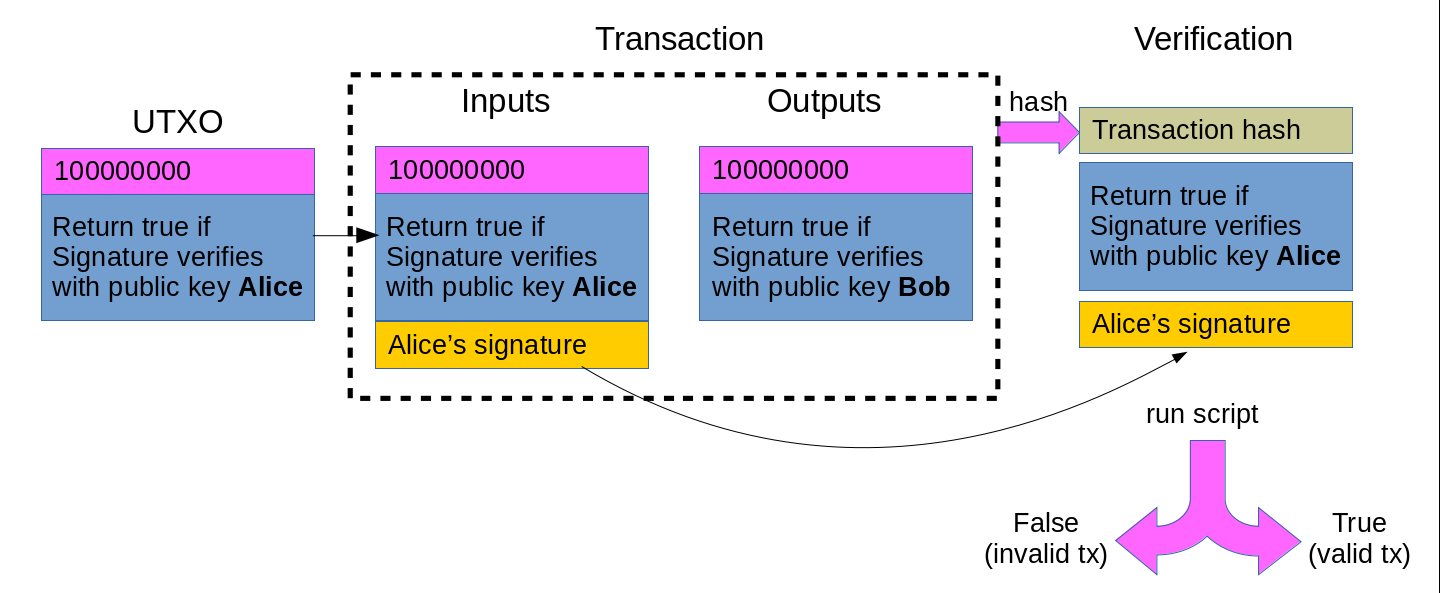
\includegraphics[scale=0.24]{bitcoin.png}
	\caption{Verifying a Bitcoin transaction}
	\label{fig1}
\end{figure}

Bitcoin's locking script can require signatures from multiple parties and also refer to context variables (the state of the blockchain). Currently, the only context variables allowed in Bitcoin are the height and time. 

Ergo is also based on the same model and a UTXO is called a {\em box} in Ergo. In addition to the amount and locking script, a box can also store additional data in {\em registers}. Ergo context has the entire spending transaction and the block solution. Thus, an Ergo contract can refer to other inputs and outputs of the transaction. For instance, we can require that certain inputs or outputs must have some structure, such as being protected by a given script. This allows creating even Turing-complete contracts~\cite{chepurnoy2018self}. 

In addition to the primary token, a box can contain some secondary tokens.
Each transaction can create arbitrary quantity of exactly one secondary token, whose id is given by the box id of the first input. Ergo follows the strong conservation rule (exactly equal) for the primary token and the weak rule (less than or equal) for secondary tokens. 

\section{One-Time Microcredit Money}
\label{sec-microcredit}

 In this section we consider a private digital scrip issued in order to serve needs of a specific credit contract.
% Thus, money behind this contract is enforced to be spent as prescribed by the precise rules of the contract.
 For example, assume that a lender in India provides a small loan to an entrepreneur for establishing a business.
 A common source of risk in this is lying during loan application, and also reckless spending of credit funds~(for example, on prestigious consumer goods instead of business tools). To reduce risks, microcredit
 organizations even conduct financial literacy trainings for clients~\cite{finliteracy}. This problem could be tackled by enforcing a borrower to spend money exactly on needs declared in the application form.  

 Assume that a borrower claims in the application form that he will spend half of a loan of $1,000,000$~(or ten lakhs) 
 Indian Rupees on equipment and $200,000$ will be spent on constructing a building where production will happen. The rest will be spent in arbitrary ways or reserved for unexpected expenses.

 The lender creates a digital token backed by Indian Rupees in 1:1 ratio, which we call IMTIR~(Individual Microcredit Token backed by Indian Rupee). Assume that there are four equipment sellers in that area known to the lender, named $E1$, $E2$, $E3$, $E4$, and three builders named $B1$, $B2$, $B3$. All the $1,000,000$ tokens are stored in one coin initially, and the coin usage is bound by the following contract:

 \begin{enumerate}
    \item{} The lender creates $1,000,000$ IMTIRs in form of a digital coin.
    \item{} When spending a coin, the borrower has to spend at least $500,000$ IMTIRs to one of $E1$, $E2$, $E3$, $E4$, and at least $200,000$ IMTIRs to one of $B1$, $B2$, $B3$. After this initial spending, IMTIRS could be spent in arbitrary way.
\end{enumerate}

 After this simple contract is done, the IMTIRs could be exchanged with Rupees, for example, via a digital asset exchange. The borrower repays the loan in Rupees as usual. 

 This basic contract could be enhanced in many ways. For example, the loan could be made interest-free. That is,
 the lender may exchange money with a discount, or introduce a demurrage~(or combine both). For example, the borrower may pay 0.97 Rupees per 1 IMTIR. Businesses would like to participate in this scheme to get an increased money flow despite the less profit. Thus, the lender may get profit from businesses and it is enough to get the loan paid out with no interest by the borrower. However, this could be the case only if the currency of the loan has no inflation. This is not the case for most fiat currencies. What the lender and borrower can do in this case is to use a trusted provider of statistical information, namely, inflation indicators. Then the lender and borrower may fix the loan using prices on the approval date.

 Then a contract\footnote{Please note that we omit the demurrage component from
 the contract.} behind IMTIR money, with the underlying interest-free loan approved on Jan, 1st, 2020,
 could be as follows: ``the borrower will pay out the debt without interest by buying IMTIR tokens with digitalized Indian Rupees, using inflation data from a trusted oracle''.
 
 In this example, IMTIR acts as contractual money bounded by the loan contract, and intentionally limited (by program code) to acts only as medium-of-exchange. A contract extended from this basic IMTIR is described in~\cite{scpeople}.

Since IMTIR token flows are public, in order to protect the lender's privacy, the borrower
 may issue tokens every month which are backed by Indian Rupees~(in prices for the beginning of the month). In our example, the borrower can repay the loan in MTIR-01-2020~(Microcredit Tokens backed by Indian Rupee in prices of
 Jan, 2020) tokens. To protect privacy of spending (to one of $B1$, $B2$, $B3$, and one of $E1$, $E2$, $E3$, $E4$), ring
 signatures~\cite{rivest2001leak} can be used. MTIR-01-2020 tokens could also be made freely tradeable~(on exchanges). 
% That is, the lender must repay the loan in 
% digitalized Rupees, and the borrower is always selling enough MTIR-01-2020 tokens for Rupees.
% , with exchange rate equals
% to, for example, official inflation since issuance of the tokens. However, if another agent is experiencing lower inflation than the borrower, he can buy at the lower price and then make profits from arbitrage.

\section{Combination of time and local currencies}
\label{sec-combination}

Local and regional currencies, such as Chiemgauer~\cite{thiel2011complementary} and Berkshares~\cite{swann1995local}, were developed to increase money flow within the local economy.
A complementary currency was proposed by Forstarter in~\cite{forstater2018complementary} as a means for local job creation by using the currency to pay for community service employment.

In this example, we show how to create a contractual currency which is intended to solve both problems of low
employment and stagnation of local economy. We will refer to this currency as LCJC (local community job currency).

For example, a local government in Russia may issue certificates, where each certificate is equals to 1 hour of community work, and also 200 Rubles. Each certificate is a digital coin, which could be converted into Rubles only by white-listed local manufactures, so a worker may spend them in any way but LCJC Rubles could be transformed into Rubles only by approved manufacturers.

In rural areas, the system could be run even without digital contracts. However, in a digital form there could be
additional properties achieved, for example,
    \begin{itemize}
        \item{} a demurrage component may be added to increase money velocity. However, demurrage can be implemented over paper 
        certificates as well, as it was done in the W\"{o}rgl experiment, but if a coin exists in digital form 
         then demurrage fee can be charged without the need to visit an office every month.
        \item{} as digital money could be traceable on the way from employers to local producers, an additional
        requirements could be made against the money flow. For example, it could be required for money to get through
        white-listed shops (from a designated list) to get to a producer. Also, it could be required for a shop, and also for a
        producer to send 1 percent of LCJC volume (each) to local charity organizations.
    \end{itemize}


With LCJC currency as a warm-up, we are ready to revisit the famous W\"{o}rgl experiment.

\section{The W\"{o}rgl Experiment}
\label{sec-worgl}

The W\"{o}rgl experiment covered in~\cite{muralt1934woergl} is a well-known successful example of a local currency. In
contrary to most of the writings suggesting that the currency was able to revive the local economy because of demurrage, we note that the experiment was a successful scheme to convert local tax debts into building community projects, with
 local businesses being fueled with money on the way. Moderate success of current regional currencies with demurrage~\cite{thiel2011complementary} is a particular sign that demurrage itself is not a silver bullet for solving problems of local economies.
 With that in mind, the original paper of Von Muralt~\cite{muralt1934woergl} is to be revisited. 

 The first question to be answered is how ``relief money''~(a term by Von Muralt) were issued. The answer from the original paper is clear: ``the depreciating money was brought into circulation by the parish paying its clerical and manual workers, at first 50\% and later 75\% of their remuneration, in relief money''. As only local businesses accepted the relief money, the scheme looks like LCJC 
 currency from the previous section. 

 However, issuance of the money did not create inflation, per Von Muralt, ``no rise in prices appears to have occurred''. The reason behind that, according to data in the paper, is that most of the money quickly returned back to parish in order to pay local tax debts. According to the paper, ``the important indirect gain of the system lies, according to the burgomaster, in that already during the first six months heavy tax arrears, 90\% of these in relief money, reached the parish treasury.'' Because of that, it became unnecessary to increase initial collateral~(in form of bank deposit) backing issued relief money. Demurrage helped businesses to pay taxes as soon as possible~(sometimes, in advance). 

 Thus, the W\"{o}rgl experiment could be represented as a scheme of converting tax debts into communal work~(such as repaired roads of the town). A contract for the experiment could be trivially stated explicitly and digitalized.

\section{Local Exchange Trading System}
\label{sec-lets}

A local exchange trading system (LETS)\cite{williams1996local} is a local mutual credit association whose members are allowed to create common credit money individually, with all the deals in the system being written into a common ledger. Usually the system is run by a committee of 
trusted managers maintaining the members list and the ledger. However, with the blockchain, global ledger functionality comes for free and we describe two blockchain-based solutions for a LETS. The first solution uses a trusted committee to manage new participants. The other solution is trustless, so anyone can join the system at any time; however, collateral in cryptocurrency is required in this case. The trustless solution is novel to the best of our knowledge.

The main difference in the two variants is the mechanism for adding new members. To describe the distinction, we recall a basic idea behind LETS. Assume that Alice and Bob have joined the system, which is using some fiat currency, for example, Euro, as unit of account. Initially
balances of both Alice and Bob are equal to 0 EUR. Now Alice wants to buy a liter of milk from Bob for 1 EUR. She creates debt on the fly, and after the deal is done her balance becomes -1 EUR while Bob's balance becomes 1 EUR. Then Bob can spend his 1 EUR on buying lettuce from Carol. Thus, LETS is about community currency emitted as IOU notes issued by community members (and notes are indistinguishable).

One of the most critical problems for LET systems is free-riding, so Alice can increase her debt as much as possible without any desire to repay it. In case of blockchain, where it is easy to create new pseudonyms, Alice can get even more by creating many identities in order to create as much debt as possible through the different identities.

There are two possibilities to avoid such free-riding. In the first option, which is more suitable for local communities, a trusted committee checks new members for possible duplicates, and also tries to convince Alice give back to the community. Often, such systems also introduce maximum debt amount for a user. Another solution is for Alice to keep collateral in cryptocurrency. Then Alice can increase her debt as long as the collateral covers it. However, as cryptocurrencies with their high volatility are not good units of account, Alice probably would like to use some more stable fiat currencies and a pricing oracle is needed. Details are provided below.

\subsection{LETS With a Trusted Committee}
\label{sec-trusted}

A LETS implementation with a trusted committee could be seen as an interaction of two contracts. The first contract, which we
call a {\em management contract}, specifies rules for adding new members. A digital coin with this contract stores system members list~(more precisely, it stores a short cryptographic digest of the list, and then a member provides a proof that he is in the list with the specified digest as and when needed). The coin also stores a committee script, for example, a threshold ($k$-out-of-$n$) signature spending condition. The coin is then protected by the combination of the committee script and requirement for a spending transaction to create a coin which is the same, except of a new record added to the members list, and maybe a new committee script~(thus a committee may also update itself, for example, by switching from 3-out-of-4 threshold signature to 4-out-of-5 in case of new committee member). The coin also requires the spending transaction to create a new member coin containing a cryptographically unique identifier of the new member~(which is also added to the members list of the management contract coin) in form of a new token issued with quantity equal to one. We refer to such a token as to a singleton token.

The second contract is an {\em exchange contract} that allows transactions between two members of the system. For that, the exchange contract requires the first two inputs of the spending transaction to be protected by the exchange contract script. The exchange contract also requires a spending input to provide a proof of membership for its coin~(which contains a singleton member token). This is possible because Ergo supports read-only inputs, and so the spending transaction needs to have the management contract coin as a read-only input. In order to be allowed to trade, a party's balance should be no less than some minimum value. The exchange contract also requires both spent inputs to be replicated as outputs with the balance changed in the proper way (decrease in balance of the sender should be accompanied with an equal increase in balance of the receiver). Note that only the sender needs to participate in the transaction. Details and code of the two contracts are provided at~\cite{lets-trusted}.


\subsection{Trustless LET System}
\label{sec-trustless}

The LET system uses a trusted committee for enrolling members. Here we consider a variant of the system without 
such a trusted committee. The main reason for having a trusted committee is to prevent the same person using duplicate identities trying to accumulate a large negative balance, thereby misusing the system. What the trusted committee does is to ensure that each real-world party can have only one LETS identity (whose negative balance can then be capped). 
 
 
Since we desire a trustless LETS, we cannot depend on any trusted group of people to admit users. We therefore allow users to accumulate a large negative balance as long as they have a certain amount of some tokens locked up as collateral. The locked amount will be adjusted automatically when the negative balance changes. Although we won't depend on a trusted committee for admitting members, we would still need a trusted oracle whose only job is to periodically emit and publish on the blockchain the exchange rate of the token with the LETS currency. 
We will also have a management committee whose job is to define the system parameters such as the pricing oracle's id, etc.

The system is designed using two contracts. The first is a {\em management contract} of which only one instance exists (i.e., it is a singleton contract). This contract is responsible for enrolling new users into the LETS. A user may enrol multiple times because this is allowed in our system. Each enrolled user is represented by an instance of a {\em membership contract}. This contract is used to perform LETS transaction and requires that any negative balance is backed by appropriate number of crypto tokens determined using the most recently emitted rate by the oracle. In order to prevent spam attacks, the system requires a joining fee which may be refunded in the form of positive LETS balance or could be collected by a management committee. 
We can envision more advanced contracts where members may buy LETS balance in exchange for crypto tokens. 
 Details and code are provided at~\cite{lets-trustless}.


\section{Concluding remarks}
\label{sec-conslusion}

In contract to paper or digital money with an external contract, less hassle is needed to use contractual money: demurrage can be paid automatically, no checks are needed to verify whether money were spent as prescribed
by its contract, and so on. Thus monies can be created and maintained in an easier way. We hope that the paper clearly shows the power of money bounded by an explicitly stated and self-enforced contract. However, with this power new possibilities for abuse also arise. In particular, corporations and governments can do even more intrusive surveillance than what simple digital monies allow. Also, monies with limited medium-of-exchange function could be used for monopolization of markets. For example, a financial corporation can provide a loan which could be spent for buying tools from a specific manufacturer only, where the corporation has a stake in the manufacturer. Such double-edged nature is typical for new technologies as they empower people with both good and bad intentions. Thus, good intentions are necessary for contractual money practitioners~(and the same is true for any new technology).

\bibliographystyle{alpha}
\bibliography{sources.bib}


\end{document}